\documentclass[a4paper,twoside]{article}

\usepackage[T1]{fontenc}
\usepackage[utf8]{inputenc}
\usepackage{epsfig}
\usepackage{subcaption}
\usepackage{calc}
\usepackage{amssymb}
\usepackage{amstext}
\usepackage{amsmath}
\usepackage{amsthm}
\usepackage{multicol}
\usepackage{pslatex}
\usepackage{apalike}
\usepackage{algorithm2e}
\usepackage[bottom]{footmisc}
\usepackage{booktabs}
\usepackage{array}
\usepackage[hidelinks]{hyperref}
\usepackage{tikz}
\usetikzlibrary{arrows.meta, decorations.markings, calc}
\usepackage{graphicx}
\usepackage{grffile}
\usepackage{SCITEPRESS}

\begin{document}
\title{Concave Hull Revisited: Runtime Analysis and Acceleration of the K-Nearest Neighbours Approach}

\author{\authorname{Sean Perman\sup{1} and Mario Lopez\sup{1}}
\affiliation{\sup{1}Ritchie School of Engineering and Computer Science, University of Denver, Denver, Colorado, U.S.A.}
\email{sean.perman@du.edu}
}

\keywords{Concave Hull, Convex Hull, Polygon, Contour, K-Nearest Neighbours, Spatial Bucketing, Computational Geometry.}

\abstract{Moreira and Santos introduced a $k$-nearest-neighbours variation of gift wrapping for constructing concave hulls. The parameter $k$ heuristically controls concavity. When construction fails, the algorithm discards the partial hull and restarts with a larger $k$ until it finds a valid hull. The original paper lacked an asymptotic runtime analysis. We show that one fixed-$k$ attempt has a worst-case upper bound of $O(kn^2)$, linear $k$-growth gives $O(n^4)$, and constant-ratio geometric growth reduces the restart bound to $O(n^3)$ under the same cost model. We also prove termination because, when all remaining points are considered, the method reduces to Jarvis march. The analysis identifies edge-intersection checking and repeated reconstruction as main costs. In a two-factor experiment on real and synthetic datasets, uniform-grid spatial bucketing gives paired median speedups of $1.40$--$3.41\times$ while preserving the ordered hull, whereas geometric growth gives $1.36$--$44.57\times$ speedups but usually selects a different valid hull. Combining both gives $1.89$--$147.94\times$ speedups over the baseline. Finally, counterexamples show that neither hull concavity nor fixed-$k$ validity is monotone in $k$, ruling out ordinary binary search for the smallest valid $k$. These results provide runtime bounds, acceleration strategies, and clarify how $k$ affects construction.}
\onecolumn \maketitle \normalsize \setcounter{footnote}{0} \vfill
% ================================================================
\section{\uppercase{Introduction}}
Given a finite set of points in the plane, many applications need a polygon that represents the region covered by those points. The convex hull is the unique smallest convex polygon containing the entire point set, and it is useful when the main goal is enclosure. However, it may not represent the shape of the data well when the points contain indentations, gaps, or separate groups. A concave hull relaxes the requirement of convexity, allowing the boundary to bend inward and follow the data more closely. Unlike the convex hull, a concave hull is not unique: many different polygons can represent the same point set with different levels of detail. Concave hull algorithms therefore use parameters or geometric rules to control the resulting boundary \cite{galton2006,duckham2008}.

Moreira and Santos proposed a concave hull algorithm based on $k$-nearest neighbours and gift wrapping \cite{moreira2007}. When the algorithm fails to construct a valid hull, it discards its partial result and starts again with a larger value of $k$. This process continues until it finds a hull containing every input point. Although the algorithm is simple and flexible, the original paper did not provide an asymptotic runtime analysis. Repeated restarts and edge-intersection checks can cause the algorithm to perform a large amount of repeated work.

This paper makes three contributions. First, we show that one attempt with fixed $k$ has a worst-case upper bound of $O(kn^2)$, and that repeated attempts under linear $k$-growth give an $O(n^4)$ upper bound. A constant-ratio geometric schedule instead gives an $O(n^3)$ upper bound under the same model. We also show that the algorithm terminates when $k$ becomes large enough to consider all remaining points. Second, we evaluate the two independent optimization targets exposed by the analysis. Uniform-grid spatial bucketing accelerates edge-intersection checking by $1.40$--$3.41\times$ without changing the hull. Geometric growth reduces the number of reconstruction attempts and gives $1.36$--$44.57\times$ speedups, while sometimes changing the selected valid hull; their combination is $1.89$--$147.94\times$ faster than the original baseline. Third, we give counterexamples showing that increasing $k$ can produce a more concave hull and that success at one value of $k$ does not imply success at every larger value.

% ================================================================
\section{\uppercase{The Moreira--Santos Algorithm}}
\subsection{Main Idea}
Moreira and Santos \cite{moreira2007} proposed a simple and intuitive concave hull algorithm based on the idea of modifying Jarvis march \cite{jarvis1973}. Instead of selecting the next hull vertex from all points, their method restricts attention to the $k$-nearest neighbours of the current vertex. Among these \textbf{candidates}, it chooses the one that creates the largest right-hand turn without introducing an intersection with the existing hull.
This restriction makes it possible to construct non-convex boundaries while preserving the local, step-by-step flavor of gift wrapping \cite{jarvis1973}. The parameter $k$ governs how local the search is: smaller values tend to produce tighter and more detailed hulls, while larger values yield smoother and more convex boundaries.

\begin{figure}[h]
  \centering
  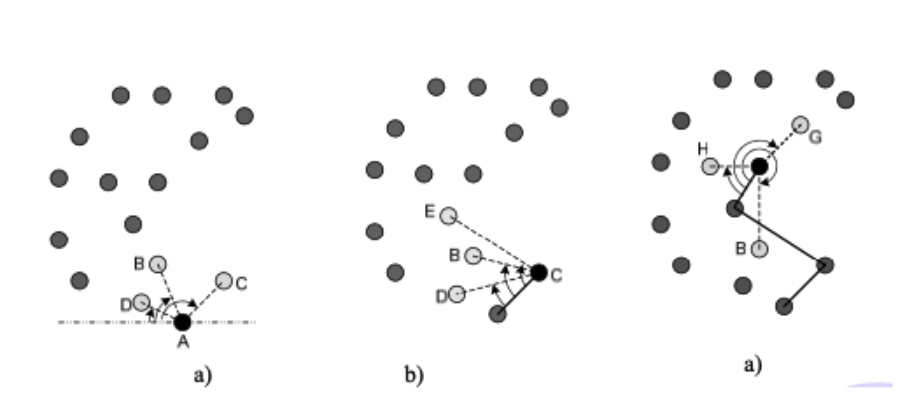
\includegraphics[width=\columnwidth]{Screenshot 2026-04-02 at 3.58.41 PM.png}
  \caption{The k-nearest neighbours approach.}
  \label{fig:knn-approach}
\end{figure}


The algorithm begins by selecting an extreme point (minimum $y$-coordinate) as the starting vertex. From the current hull vertex, it computes the $k$-nearest neighbours that have not been excluded from consideration. These candidates are then ordered according to the turning angle relative to the previous hull edge. A greedy approach is then used to select a \textbf{valid candidate} that produces the largest right-hand turn without intersecting the existing hull. This process repeats until the walk returns to the starting point, thereby closing the polygon.

\subsection{Failure Cases and Restart Logic}
\begin{figure}[h]
  \centering
  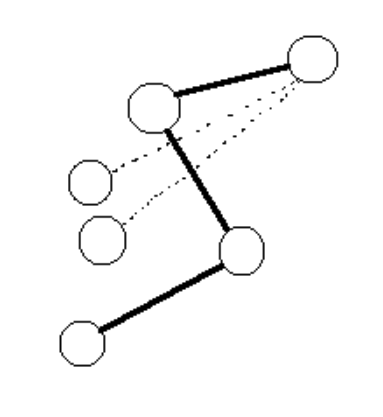
\includegraphics[width=0.6\columnwidth]{Screenshot 2026-04-02 at 3.53.56 PM.png}
  \caption{All candidate edges intersect the current hull.}
  \label{fig:dead-end}
\end{figure}
The algorithm has two main failure cases. First, there may be no valid candidates among the current $k$-nearest neighbours: each candidate edge intersects the existing partial hull, so the algorithm cannot safely extend the boundary (\textbf{dead end}). Second, after the hull has been closed, some input points may still remain outside the polygon. In that case, the computed hull fails to enclose the full point set (\textbf{excluded points}).
\subsection{The Role of the Parameter $k$}
The parameter $k$ is the central control variable in the algorithm. When $k$ is small, candidate selection is highly local, allowing the boundary to follow fine geometric detail and concave features. When $k$ is larger, the set of candidate vertices broadens, and the resulting hull tends to be smoother and closer to a convex enclosure. In the case where $k=n$, large enough that all remaining points are considered at each step, the method is identical to the Jarvis-march search and produces the convex hull.
\begin{figure}[h]
  \centering
  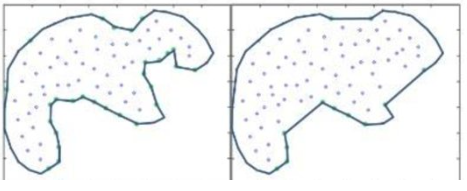
\includegraphics[width=1\columnwidth]{Screenshot 2026-04-02 at 4.04.57 PM.png}
  \caption{(left = low $k$), (right = high $k$).}
  \label{fig:k-comparison}
\end{figure}
An important feature of the method is that $k$ is dimensionless: it is not a geometric distance threshold, but rather a count of neighbours. This distinguishes it from approaches such as alpha shapes, where the main parameter is directly tied to spatial scale and may be sensitive to sampling density \cite{edelsbrunner1983}. In the Moreira--Santos method, the parameter has a more combinatorial interpretation, which can make it easier to reason about across differently scaled datasets.
\subsection{Comparison with Other Concave Hull Approaches}
Compared with alpha-shape-based methods and related shape reconstruction techniques, the Moreira--Santos algorithm has the advantage of conceptual simplicity and a parameter that is not directly tied to metric scale. In contrast, methods based on geometric thresholds often require careful tuning relative to point spacing or sampling density \cite{edelsbrunner1983,liao2021}.
The k-nearest-neighbours approach is therefore appealing both practically and theoretically. It offers a direct geometric construction, adapts automatically by increasing $k$ when necessary, and provides a natural bridge between highly detailed concave boundaries and more convex approximations. These properties make it a useful baseline for the improvements developed in the later sections of this paper.
% ================================================================
\section{\uppercase{Runtime Analysis of the Original Algorithm}}
\subsection{Cost of One Successful or Failed Run with Fixed $k$}
We first analyze one execution of the original Moreira--Santos algorithm with a fixed neighbour parameter $k$. Let $n$ denote the number of input points, and let $s$ denote the number of steps completed before that run either closes a hull or fails and triggers a restart. Since each non-closing step adds a new hull vertex and removes a point from further consideration, we have $s = O(n)$.
At each step, the algorithm performs three main operations:
\paragraph{Nearest-neighbour search.}
At each step, the algorithm computes the $k$-nearest neighbours of the current point. The original paper's Mathematica package invokes a helper named \texttt{NearestPoints}; it specifies Euclidean distance, but neither identifies this helper as a Wolfram built-in nor reports its data structure or selection algorithm \cite{moreira2007}. To give the implementation the benefit of the doubt, we model exact neighbour selection as linear and charge no separate index-construction or rebuilding cost:
\[
T_{\mathrm{knn}}(i)=O(n).
\]
This is also a valid worst-case bound for exact tree-based search. Granting the more optimistic expected indexed-query cost $O(\log n+k)$ would only reduce the nearest-neighbour contribution; the intersection term derived below would still dominate.
\paragraph{Sorting the candidates.}
Once the $k$ nearest neighbours have been selected, they are sorted by angle relative to the previous hull direction. Sorting $k$ items costs
\[
T_{\mathrm{sort}}(i)=O(k\log k).
\]
\paragraph{Intersection checking.}
Suppose the partial hull currently contains $i$ vertices. A candidate edge must be checked against $O(i)$ existing hull edges. Since the algorithm may test as many as $k$ candidates before finding a valid one or concluding that no valid candidate exists, the intersection-checking cost at step $i$ is
\[
T_{\mathrm{check}}(i)=O(k\,i).
\]
Therefore, the total cost at step $i$ is
\[
T(i)=O(n)+O(k\log k)+O(k\,i).
\]
Summing over all $s$ steps in the run gives
\[
C_{\mathrm{run}}(k)
=
\sum_{i=1}^{s}\Bigl(O(n)+O(k\log k)+O(k\,i)\Bigr).
\]
Separating the three contributions:
\[
C_{\mathrm{run}}(k)
=
O(sn)+O(sk\log k)+O\!\left(k\sum_{i=1}^{s} i\right).
\]
Using the triangular-sum identity, $\sum_{i=1}^{s} i = O(s^2)$, we obtain
\[
C_{\mathrm{run}}(k)=O(sn)+O(sk\log k)+O(ks^2).
\]
Since $s = O(n)$, this yields
\[
C_{\mathrm{run}}(k)=O(n^2)+O(nk\log k)+O(kn^2).
\]
A completed run also performs a final containment check to verify that all points lie inside the constructed polygon. In the worst case, this adds at most $O(n^2)$, which does not change the asymptotic bound above.
Since $k \ge 1$, the term $O(kn^2)$ dominates, giving a single run with fixed $k$ worst-case cost:
\[
\boxed{C_{\mathrm{run}}(k)=O(kn^2).}
\]
\subsection{Cost of Restarts}
The original algorithm may restart with a larger value of $k$ in two cases: first, when all current candidates would produce an intersecting edge (\textbf{dead end}), and second, when a closed hull is found but at least one input point lies outside the resulting polygon (\textbf{excluded points}). In either case, the algorithm discards the current hull and restarts from the beginning with $k+1$.
Suppose the algorithm begins with $k_0$ and eventually succeeds only after trying the sequence $k_0, k_0+1, k_0+2, \dots, K$. Then the total cost is:
\[
C_{\mathrm{total}}
=
\sum_{k=k_0}^{K} C_{\mathrm{run}}(k)
=
O\!\left(n^2 \sum_{k=k_0}^{K} k\right).
\]
In the worst case, the algorithm restarts may increase $k$ until $K=n-1$. Therefore,
\[
C_{\mathrm{total}}
=
O\!\left(n^2 \sum_{k=1}^{n-1} k\right)
= O(n^2 \cdot n^2)
= \boxed{O(n^4).}
\]

This bound depends on the original linear update $k\leftarrow k+1$. Consider
instead a constant-ratio geometric schedule
\[
k_{j+1}=\min\{\lceil r k_j\rceil,n-1\},\qquad r>1.
\]
The tested values form a geometric series, so $\sum_j k_j=O(n)$. Applying the
same per-run bound gives
\[
C_{\mathrm{geo}}
=O\!\left(n^2\sum_j k_j\right)
=\boxed{O(n^3)}.
\]
This is an upper bound for a modified growth schedule, not for the original
algorithm. The schedule may skip smaller successful values of $k$ and therefore
change the returned hull, but it remains terminating when the all-candidates
value is used as an explicit cap.
These bounds identify two independent optimization targets. Within an attempt,
edge-intersection checking drives the $O(kn^2)$ term; across attempts, the growth
schedule determines the restart sum. Section~4 addresses the first target with
spatial bucketing. Geometric growth addresses the second, but may skip smaller
successful values of $k$; Section~6 shows that ordinary binary search cannot
recover the minimum in general because fixed-$k$ validity is not monotone.
% ================================================================


\subsection{Termination}

The original paper states that repeatedly increasing \(k\) eventually produces a valid hull, but its pseudocode does not establish this for every input. The value of \(k\) is capped at \(n-1\), yet a failed attempt at that value recursively calls the algorithm with \(k+1\), which is immediately reduced back to \(n-1\). The same failed attempt may therefore be repeated indefinitely. This is an oversight in the original termination argument: boundedness of \(k\) alone does not imply termination, particularly for degenerate inputs such as fully collinear point sets, which do not admit a two-dimensional polygonal hull. For point sets in general position whose convex hull has at least four vertices, termination can instead be established by showing that the \(k=n-1\) attempt follows Jarvis march, closes the convex hull, and cannot trigger another restart.

TODO: Add the formal termination proof. 


\section{\uppercase{Spatial Bucketing Improvement}}

The runtime analysis identifies edge-intersection checking as one of the main costs within each construction attempt. When the partial hull contains \(h\) edges, a naive implementation may compare every candidate edge against all \(h\) existing edges. Many of these comparisons are unnecessary because an edge located far from the candidate cannot intersect it. We reduce this work using uniform-grid spatial bucketing, a standard technique for limiting geometric tests to nearby objects \cite{franklin1989}.

The method divides the plane into square grid cells. When an edge is added to the hull, a reference to it is stored in every cell containing any part of that edge. When testing a new candidate edge, the algorithm looks at the cells containing the candidate and applies the exact intersection test only to the existing hull edges referenced in those cells. An existing edge referenced in multiple cells is checked only once. Because intersecting edges share at least one cell, this filtering does not miss any intersections. Points on grid boundaries are associated with the adjacent cells so that boundary intersections are also detected.

For the experiments, the grid-cell width is selected automatically as

\[
w=\frac{\max\{\Delta_x,\Delta_y\}}{\sqrt{n}},
\]

where \(\Delta_x\) and \(\Delta_y\) are the coordinate ranges of the input and \(n\) is the number of input points. This choice scales the grid according to both the spatial extent of the data and the number of points.

Let \(g\) be the number of grid cells containing part of a candidate edge, and let \(i\) be the number of distinct existing hull edges retrieved from those cells. Assuming constant-time grid lookups, processing one candidate requires \(O(g+i)\) work, including the exact tests against the retrieved edges. In comparison, the naive implementation may require \(O(h)\) exact tests. The worst-case bound is unchanged because \(i\) can still be as large as \(h\). For spatially distributed hull edges, however, \(i\) is usually much smaller than \(h\). Spatial bucketing is therefore a practical reduction in intersection work rather than an improvement to the worst-case complexity class. Section~\ref{sec:experiments} evaluates its effect on intersection counts and running time.

\section{\uppercase{Experimental Evaluation}}
\label{sec:experiments}

\begin{figure*}[h]
  \centering
  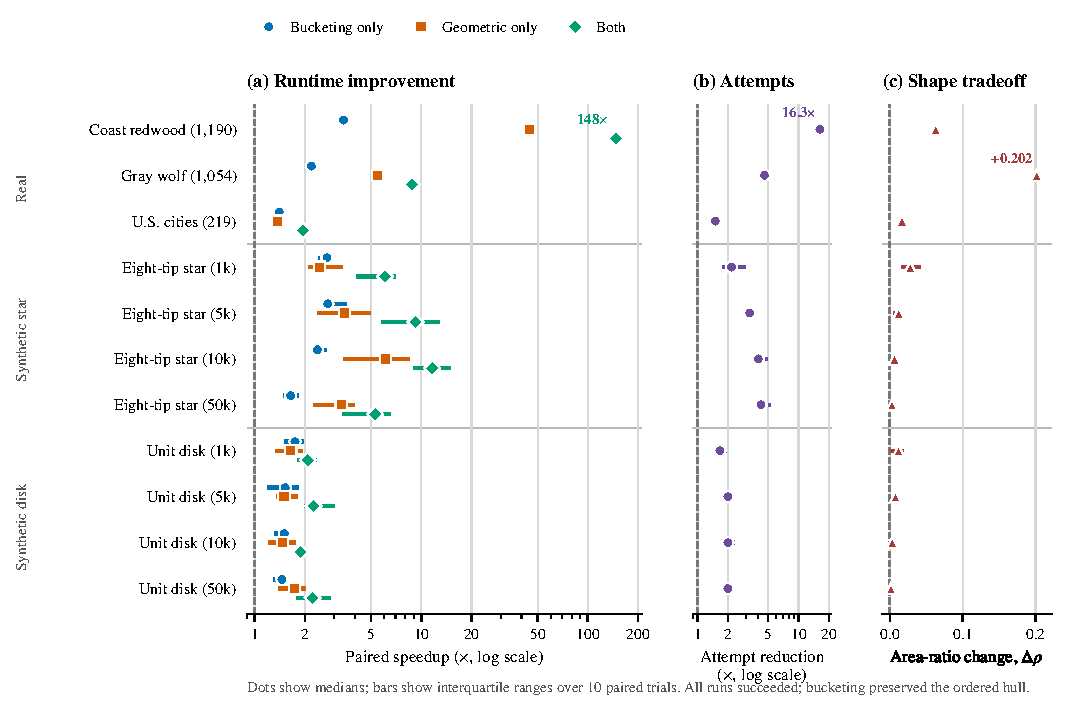
\includegraphics[width=\textwidth]{figures/growth_factorial_results.pdf}
  \caption{Results of the $2\times2$ factorial experiment. Speedups are relative
  to the original linear-growth, naive-intersection baseline. Dots show medians
  and bars show interquartile ranges over ten paired trials. Attempt reduction
  compares linear and geometric growth; attempts include the final successful
  construction, so attempts equal restarts plus one. The area-ratio change is
  $\Delta\rho=\rho_{\mathrm{geometric}}-\rho_{\mathrm{linear}}$; positive values
  indicate a larger enclosed area, not necessarily a higher-quality hull. All
  runs produced valid hulls, and bucketing preserved the ordered hull.}
  \label{fig:growth-factorial-results}
\end{figure*}


We implemented a configurable version of the original algorithm and evaluated two changes: spatial bucketing and geometric growth of \(k\). Spatial bucketing replaces the naive scan of all hull edges, while geometric growth replaces the original update rule \(k \leftarrow k+1\) with
\[
k \leftarrow \min\{\lceil 2k\rceil,n-1\}.
\]
Combining these choices produces four configurations: the original algorithm, bucketing only, geometric growth only, and both improvements together.

To ensure a fair comparison, all four configurations begin with \(k_0=3\), use the same SciPy \texttt{cKDTree} nearest-neighbour implementation, restart after an unsuccessful construction attempt, and require the final hull to contain every input point.

We used three real geographic datasets: contiguous U.S. cities ($n=219$), gray-wolf
sightings ($n=1054$), and coast-redwood sightings ($n=1190$). We also used points
sampled uniformly from a disk, as in the original paper~\cite{moreira2007}, and an
eight-pointed star designed to create difficult concavities and force dead ends. Each
synthetic family was tested at $n=1{,}000$, $5{,}000$, $10{,}000$, and $50{,}000$
over ten random seeds; each real dataset received ten timing trials.

Every trial evaluated all four configurations on the same input, and their execution order was varied across trials to reduce timing bias. An untied warm-up preceded each timing series to exclude one-time library-loading costs, and intersection counts were collected separately so that counting did not affect the runtime measurements. For each run, we measured runtime, the number and values of \(k\) tested, the final \(k\), and the number of exact intersection tests. We also computed the hull area ratio \(\rho\) and verified that the final hull contained every input point. Within each growth schedule,
naive and bucketed checking produced identical ordered hulls in all 220
schedule-matched comparisons.


Figure~\ref{fig:growth-factorial-results} summarizes the paired results. Bucketing alone gives paired
median speedups of $1.40$--$3.41\times$ and reduces exact-intersection predicates by
$6.9$--$188.6\times$. Geometric growth gives $1.36$--$44.57\times$ speedups with
naive checking and $1.21$--$43.52\times$ with bucketing. It reduces the number of
attempts by $1.5$--$16.3\times$ and the sum of tested $k$ values by
$1.33$--$17.80\times$. Combining both changes gives $1.89$--$147.94\times$ speedups
over the original baseline.

Geometric growth is not quality-preserving in the same sense as bucketing: it skips
values of $k$. It returned the same hull as linear growth in only 11 of 110 paired
inputs. In this experiment the other 99 hulls had larger $\rho$, and the median
dataset-level increase ranged from $0.003$ to $0.202$. For coast redwood, for example,
the median attempt count falls from 114 to 7, while final $k$ rises from 116 to 192
and $\rho$ rises from $0.359$ to $0.422$. These observations establish a practical
runtime--shape tradeoff, not a monotone relationship between $k$ and concavity.

\section{\uppercase{Non-Monotone Effects of $k$}}
The parameter $k$ is usually described as a smoothness control: a larger value
broadens the candidate set and tends to produce a boundary closer to the convex
hull. There are two distinct monotonicity questions. First, does increasing $k$
always make a valid hull less concave? Second, if a fixed-$k$ attempt is valid,
must every larger value also be valid? We give counterexamples to both claims.

\begin{figure*}[h]
  \centering
  \begin{subfigure}[t]{0.42\textwidth}
    \centering
    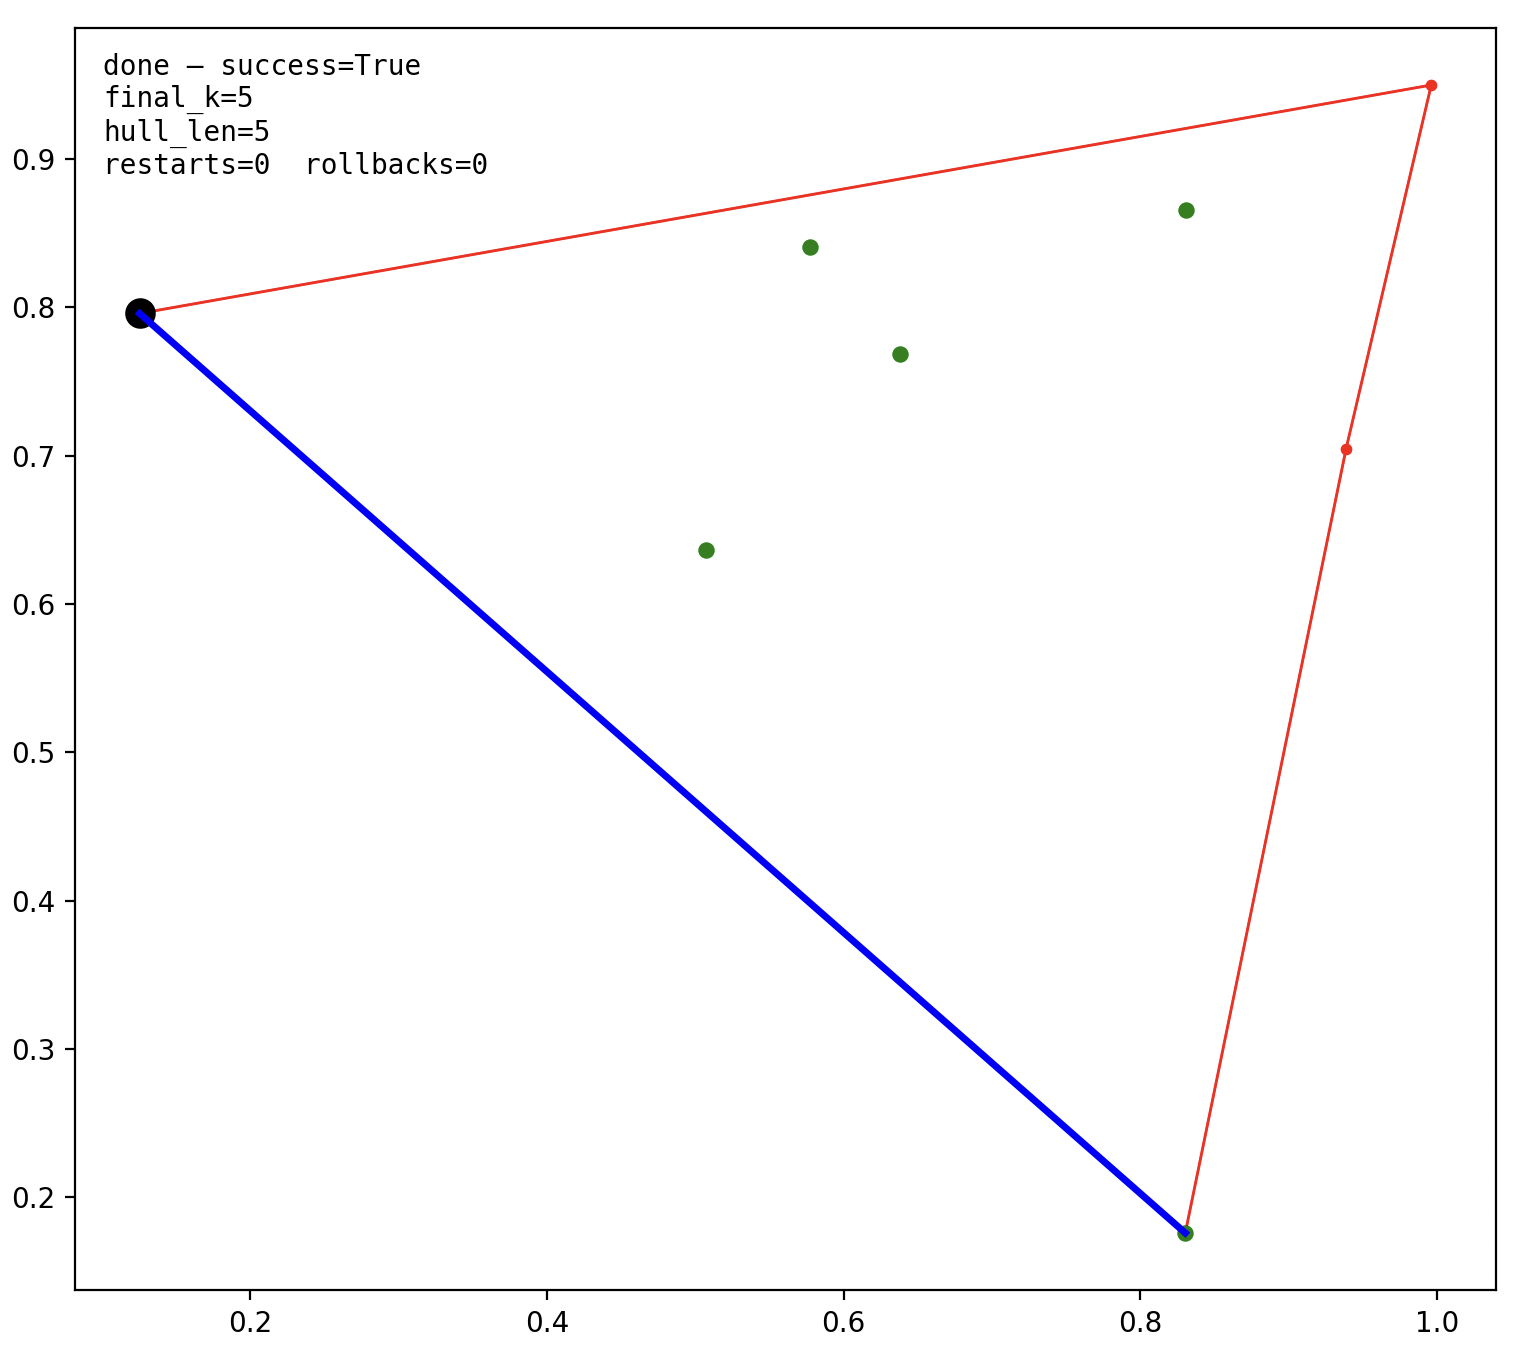
\includegraphics[width=\linewidth]{Screenshot 2026-06-16 at 11.23.01 AM.png}
    \caption{$k=5$: $\rho\approx0.9942$.}
  \end{subfigure}\hfill
  \begin{subfigure}[t]{0.42\textwidth}
    \centering
    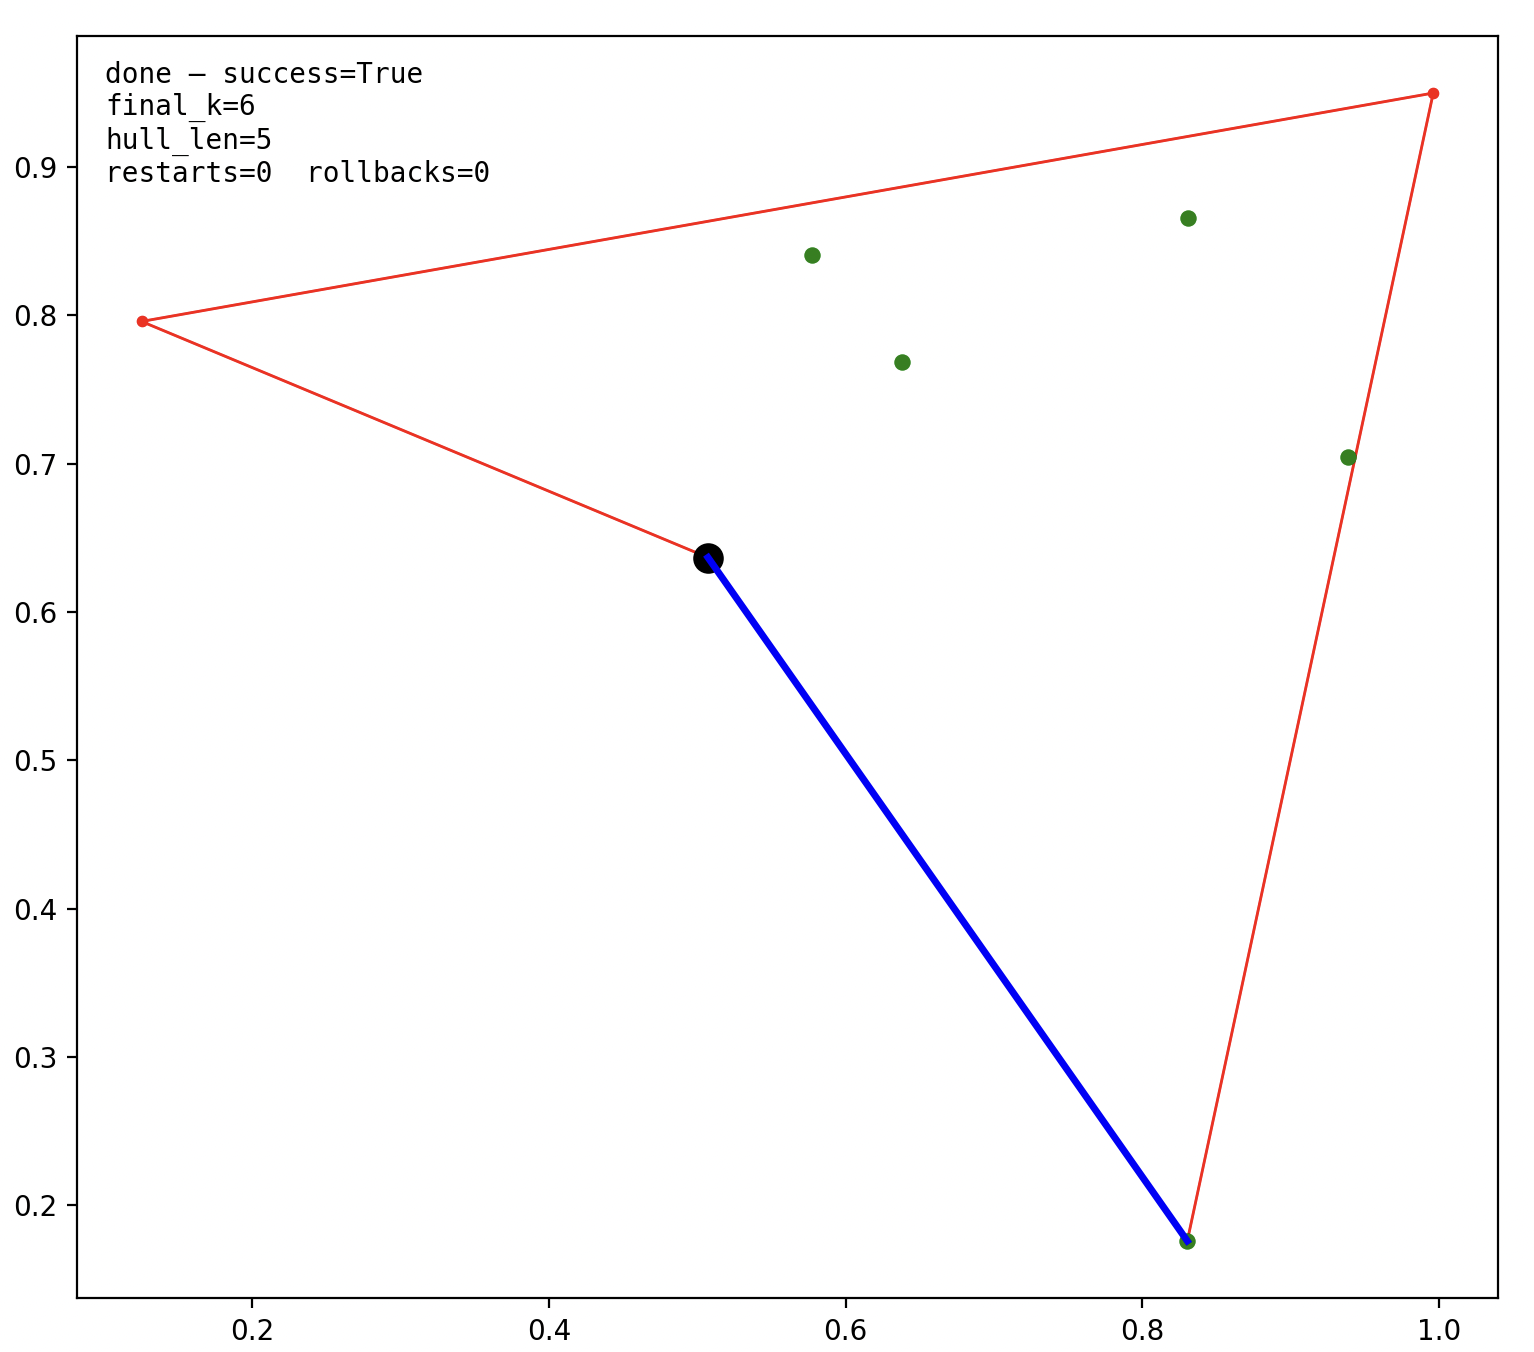
\includegraphics[width=\linewidth]{Screenshot 2026-06-16 at 11.24.21 AM.png}
    \caption{$k=6$: $\rho\approx0.8079$.}
  \end{subfigure}
  \caption{Increasing $k$ can produce a more concave valid hull.}
  \label{fig:shape-counterexample}
\end{figure*}

\subsection{Hull Shape Is Not Monotone}
For a valid hull $H$ of a point set $S$, define the area ratio
\[
\rho(H)=\frac{\operatorname{area}(H)}
{\operatorname{area}(\operatorname{conv}(S))},\qquad 0<\rho(H)\leq 1.
\]
Smaller values mean that the boundary removes more empty area from the convex
hull. For the eight-point set in Table~\ref{tab:ce-points}, the convex-hull area
is $0.32411$. The algorithm gives
\begin{align*}
\rho(H_5)&=\frac{0.32223}{0.32411}\approx0.9942,\\
\rho(H_6)&=\frac{0.26187}{0.32411}\approx0.8079.
\end{align*}
Both hulls enclose all eight input points, but increasing \(k\) from 5 to 6 produces the more concave hull shown in Figure~\ref{fig:shape-counterexample}. With \(k=6\), the algorithm can consider an additional neighbor and therefore skips a nearby point early in the construction. That point remains available and is selected later, pulling the boundary inward and creating a deeper concavity. Increasing \(k\) can therefore change the order in which points are selected rather than simply making the same hull smoother.

\begin{table}[h]
  \centering
  \caption{Eight-point shape counterexample.}
  \label{tab:ce-points}
  \begin{tabular}{cc@{\qquad}cc}
    \toprule
    \(x\) & \(y\) & \(x\) & \(y\) \\
    \midrule
    0.99603 & 0.94980 & 0.93863 & 0.70464 \\
    0.12534 & 0.79581 & 0.63777 & 0.76837 \\
    0.83024 & 0.17598 & 0.83103 & 0.86563 \\
    0.57695 & 0.84059 & 0.50715 & 0.63669 \\
    \bottomrule
  \end{tabular}
\end{table}



\subsection{Fixed-\(k\) Validity Is Not Monotone}

Let \(V(k)\) be true when a fixed-\(k\) attempt successfully constructs a hull that encloses all input points. One possible way to find the smallest valid \(k\) would be binary search. However, binary search would require a single validity threshold: values below the threshold would fail, while the threshold and every larger value would succeed.

The following six-point integer set shows that this requirement does not hold:
\[
\begin{split}
S_v=\{&A=(9,9),\ B=(7,9),\ C=(0,2),\\
      &D=(0,8),\ E=(4,7),\ F=(3,1)\}.
\end{split}
\]
The set has no three collinear points, and no point has two neighbours at the same distance. The result therefore does not depend on geometric degeneracy or nearest-neighbour tie-breaking. Direct execution gives
\[
V(3)=\mathrm{true},\qquad
V(4)=\mathrm{false},\qquad
V(5)=\mathrm{true}.
\]

At \(k=3\), the walk
\(F\to E\to A\to B\to D\to C\to F\)
closes and contains all six points. At \(k=4\), the walk begins
\(F\to B\to A\), but every possible continuation from \(A\) to \(C\), \(D\), or \(E\) intersects the existing edge \(FB\). The construction therefore reaches a dead end. At \(k=5=n-1\), the walk
\(F\to A\to B\to D\to C\to F\)
closes and encloses \(E\). Figure~\ref{fig:validity-counterexample} shows these three outcomes.

\begin{figure*}[t]
  \centering
  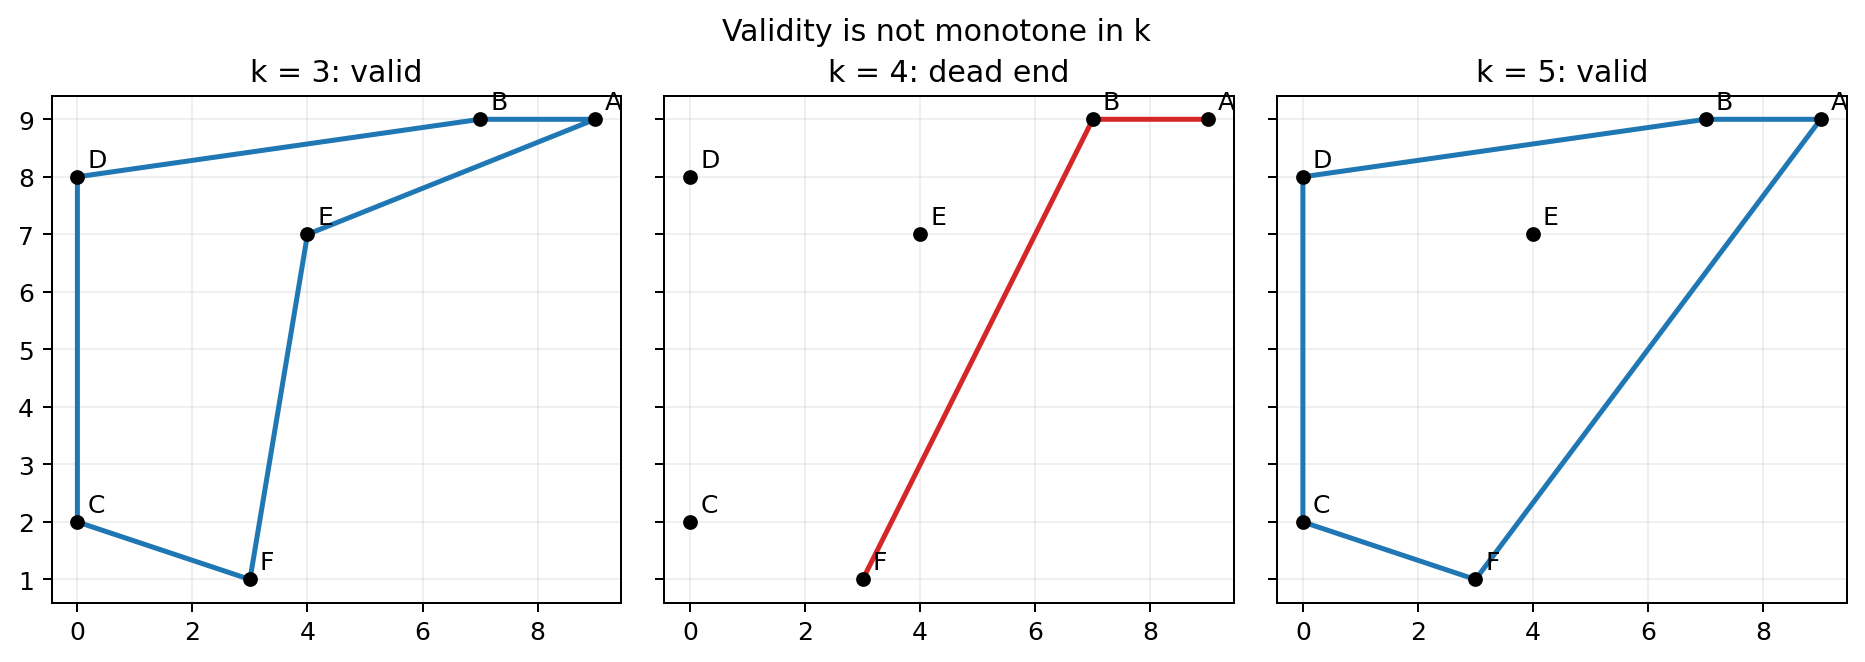
\includegraphics[width=0.94\textwidth]{../validity_monotonicity/counterexample.png}
  \caption{A six-point validity counterexample. The fixed-\(k\) construction is
  valid at \(k=3\), fails at \(k=4\), and is valid again at \(k=5\).}
  \label{fig:validity-counterexample}
\end{figure*}

These outcomes show that fixed-\(k\) validity is not monotone. Binary search is therefore not a correct method for finding the smallest valid \(k\): after observing the failure at \(k=4\), it could discard smaller values even though \(k=3\) succeeds. The geometric schedule does not require validity to be monotone. It simply increases \(k\) after each failed attempt until it finds a valid hull or reaches \(k=n-1\), where all remaining points are considered. Geometric growth may skip a smaller successful value, but it still progresses toward the guaranteed all-candidates result.


% ================================================================
\section{\uppercase{Future Work}}

\paragraph{Reducing discarded work.}
The restart analysis shows that an unsuccessful attempt discards the entire
partial hull and repeats the construction with a larger value of \(k\). An
alternative would be to save the partial hull at selected points and, after a
failure, return to one of these points and rebuild only the affected portion of
the boundary. We refer to this partial-restart approach as \emph{checkpoint
trimming}. A complete treatment would need to determine where checkpoints
should be placed, how to recover when a closed hull excludes points, and how to
preserve containment and termination.

\paragraph{Amortized analysis of the full algorithm.}
The current analysis bounds each construction attempt separately and then sums
those bounds across the tested values of \(k\). An amortized analysis could
instead track the total work spent constructing, testing, discarding, and
reconstructing hull edges over the complete execution. This could provide a
tighter description of the original restart algorithm and determine whether
checkpoint trimming improves the asymptotic runtime or primarily reduces
practical wasted work.

\paragraph{Candidate-selection criteria.}
A complementary direction is to reduce the number of failures that trigger
reconstruction. The current algorithm selects candidates using proximity and
turning angle. Alternative criteria could also consider distance, local point
density, intersection risk, or the position of the remaining points. These
criteria could be evaluated by measuring their effects on failed attempts,
discarded work, total runtime, and the shape of the resulting hull.
\section{\uppercase{Conclusion}}
We revisited the Moreira--Santos k-nearest neighbours concave hull algorithm to
explain its cost and improve its practical performance. One fixed-$k$ attempt has
an $O(kn^2)$ worst-case upper bound, while the original linear restart rule gives
an $O(n^4)$ upper bound. Constant-ratio geometric growth changes the restart sum
and lowers the corresponding upper bound to $O(n^3)$, although it may skip smaller
successful values of $k$.

Uniform-grid spatial bucketing reduces exact intersection predicates without
changing the resulting hull; across the tested real and synthetic datasets it
produced paired median speedups of $1.40$--$3.41\times$ over naive checking.
Geometric growth reduced attempts by $1.5$--$16.3\times$ and produced
$1.36$--$44.57\times$ speedups, while usually selecting a different valid hull.
The combined configuration was $1.89$--$147.94\times$ faster than the original
linear-growth, naive-intersection baseline.
Finally, $k$ is not a monotone control variable. A larger value can produce a
more concave valid hull, and fixed-$k$ validity can change from true to false and
back to true. The latter result rules out ordinary binary search for the smallest
valid $k$, while leaving forward geometric growth as a terminating alternative.
% ================================================================
\bibliographystyle{apalike}
{\small
\bibliography{references}}
\end{document}
